\chapter{Introduction} \label{sec:introduction}
    \pagenumbering{arabic}
    %\rfoot{\iffloatpage{}{\footnotesize \thepage\ of \pageref{LastPage}}}
    \rfoot{\footnotesize \thepage\ of \pageref{LastPage}}

    % Opening introductory 1/2/3 paragraphs to setup thesis.
    % Paragraph to ouline the rest of the chapter.

    % Use ideas from FGR and PE to motivate the thesis.

    % \lettrine[lines=3]{\color{UoNBlue1}T}{his}
    This thesis utilises a mathematical model of maternal blood flow and oxygen concentration in the at-term human placenta, using a physiologically-informed 2D organ-scale geometry. The solutions are approximated using discontinuous Galerkin finite element methods from the existing numerical literature. The three main contributions of this thesis are to use the aforementioned model and numerics to investigate how placental structure influences flow and transport, to model MRI scans of flow, and to introduce a preliminary model of the newly-discovered utero-placental pump phenomenon.

    The remainder of this chapter presents a literature review of placental physiology and existing placental mathematical modelling.

    % 1.1 Placental physiology
    \section{Placental physiology}
        % To cover: structure and function in detail (concentrating on aspects of most relevance to the thesis). Touch on biomechanics and potential importace.
        % Diseases, and link back to relevance in this thesis.

        % Overview of placenta
        The placenta is a crucial organ that is essential for our birth. It is unique in that it can be straightforwardly examined ex vivo after delivery, enabling, for example, convenient ex vivo perfusion experiments to investigate placental function \cite{lewisPlacentalPerfusionMathematical2020,nyeHumanPlacentalOxygenation2018}. The role of the placenta is detailed by \citeauthor{jensenBloodFlowTransport2019} in \cite{jensenBloodFlowTransport2019}. In summary, the placenta has two main purposes: facilitating the transport of oxygen and nutrients from the mother to the fetus, and transporting carbon dioxide and waste products from the fetus to the mother. In human placentas, fetal blood flows through villous trees that are submerged in maternal blood, which flows through the surrounding intervillous space (IVS). Fetal and maternal blood do not directly mix: exchange between fetal and maternal blood takes place through the large surface area of the villous tree.

        % What does a placenta look like? Function; size and weight; structure.
        A healthy delivered placenta is usually disk-like with a typical diameter of \qty{22}{\centi\meter}, thickness of \qty{2.5}{\centi\meter}, and weight of \qty{470}{\gram} at full-term \cite{benirschkePathologyHumanPlacenta2012}. However, the in vivo measurements conducted by \citeauthor{afrakhtehCorrelationPlacentalThickness2013} \cite{afrakhtehCorrelationPlacentalThickness2013} using ultrasound have reported a larger average thickness of approximately \qty{3.6}{\centi\meter}, the disparity arising due to leakage of maternal blood and a pressure drop in the IVS after delivery, resulting in a collapse of placental structure and decrease in placental volume \cite{lecarpentierComputationalFluidDynamic2016,afrakhtehCorrelationPlacentalThickness2013}. Structurally, the placenta comprises many smaller functional units, partially separated from one another by so-called \textit{septal walls} or \textit{septa}. Naming conventions for these functional units differ between authors, with common words often found in the literature being \textit{lobe}, \textit{lobule}, \textit{cotyledon}, and \textit{placentone} \cite{kaufmannPlacentalVascularizationBlood1988}. The largest unit is called a \textit{lobe}, of which there are approximately $4$--$6$, with each \textit{lobe} containing approximately $8$--$10$ \textit{lobules}. An average healthy placenta is expected to contain between $30$ and $60$ \textit{lobules} \cite{serovRoleMorphologyMathematical2016,benirschkePathologyHumanPlacenta2012,kaufmannPlacentalVascularizationBlood1988}. \textit{Lobes} are distinguished by taller surrounding septal walls compared to \textit{lobules}, with recent measurements of the smaller and taller wall heights to respectively be on average \qty{6.90}{\milli\meter} and \qty{14.07}{\milli\meter} \cite{AMANITIS2023e68}. \textit{Placentones} are idealised units that correspond to one \textit{lobule} containing one villous tree \cite{kaufmannPlacentalVascularizationBlood1988,jensenBloodFlowTransport2019}. Placentones in the interior of the placenta are generally accepted to be approximately \qty{40}{\milli\meter} in diameter \cite{chernyavskyMathematicalModelIntervillous2010,lecarpentierComputationalFluidDynamic2016}, with smaller placentones as small as \qty{10}{\milli\meter} in diameter at the placental margin \cite{benirschkePathologyHumanPlacenta2012}. Figure \ref{fig:placenta:lobules} highlights lobes and lobules on the maternal side of a delivered placenta (i.e., the basal plate). For consistency, for the remainder of this thesis we will employ the terminology \textit{placentones} to denote all functional units surrounded by septal walls of any height.

        % Structure and vessels.
        Figure \ref{fig:placenta:cartoon} shows the structure of the placenta, with the maternal blood supply entering and exiting at the bottom, and the fetal blood supply entering and exiting at the top. Spiral arteries are the name given to maternal arteries entering the placenta. Brosens wrote in 1988 \cite{kaufmannPlacentalVascularizationBlood1988} that they found most spiral arteries were found on the basal plate or in the lower third of a septal wall, and estimated a total of 120 arterial openings over the entire placenta; there has also been evidence of chorionic veins \cite{benirschkePathologyHumanPlacenta2012}, and $5$--$6$ larger muscular veins thought to encircle the placenta, providing additional drainage \cite{nanaevHumanPlacentaEncircled2000}. The exact number of arteries and veins in a placenta may significantly vary from placenta to placenta, with current literature suggesting there to be $30$--$150$ arteries and $50$--$200$ veins for the maternal blood \cite{benirschkePathologyHumanPlacenta2012,chernyavskyMathematicalModelIntervillous2010,burtonRheologicalPhysiologicalConsequences2009}. Whilst several studies have focussed on maternal arterial flow (e.g., \cite{burtonRheologicalPhysiologicalConsequences2009,jamesTrophoblastPlugsImpact2018,saghianAssociationPlacentalJets2017,collinsDevelopmentalChangesSpiral2012}), few studies have considered the venous drainage, despite this being critical to the circulation of maternal blood, and therefore delivery of oxygen and nutrients \cite{hutchinsonFirstVivoDemonstration2020}. Furthermore, the location of vessels is not well understood; \citeauthor{chernyavskyMathematicalModelIntervillous2010} \cite{chernyavskyMathematicalModelIntervillous2010} outline the three main hypotheses for vein locations: random; concentrated near the placental margins, and concentrated near the placental septa \cite{boydHumanPlacenta1970}.

        \begin{figure}
            \thisfloatpagestyle{empty}
            \centering
            \begin{subfigure}[b]{0.6\textwidth}
                \centering
                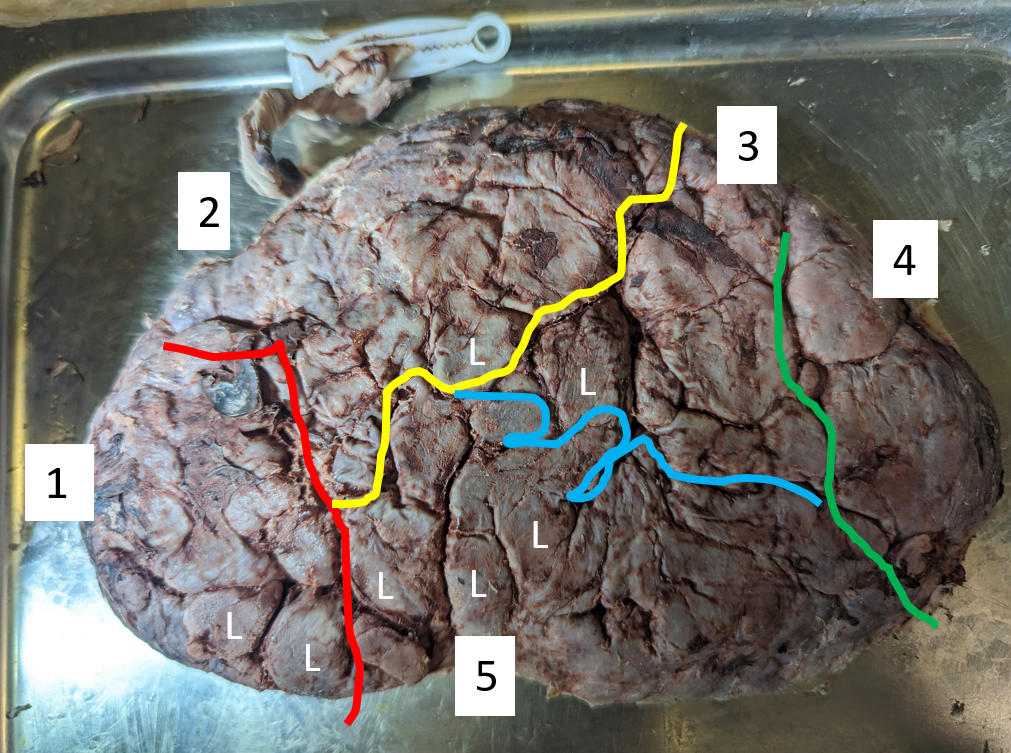
\includegraphics[width=\textwidth]{diagrams/real-placenta-pictures/placenta-lobules.png}
                \caption{}
                \label{fig:placenta:lobules}
            \end{subfigure}
            \hfill
            \begin{subfigure}[b]{\textwidth}
                \centering
                

\tikzset{every picture/.style={line width=0.75pt}} %set default line width to 0.75pt        
\resizebox{\textwidth}{!}{%
\begin{tikzpicture}[x=0.75pt,y=0.75pt,yscale=-1,xscale=1,font=\sffamily]
%uncomment if require: \path (0,435); %set diagram left start at 0, and has height of 435

%Image [id:dp612682770859811] 
\draw (251.86,178.3) node  {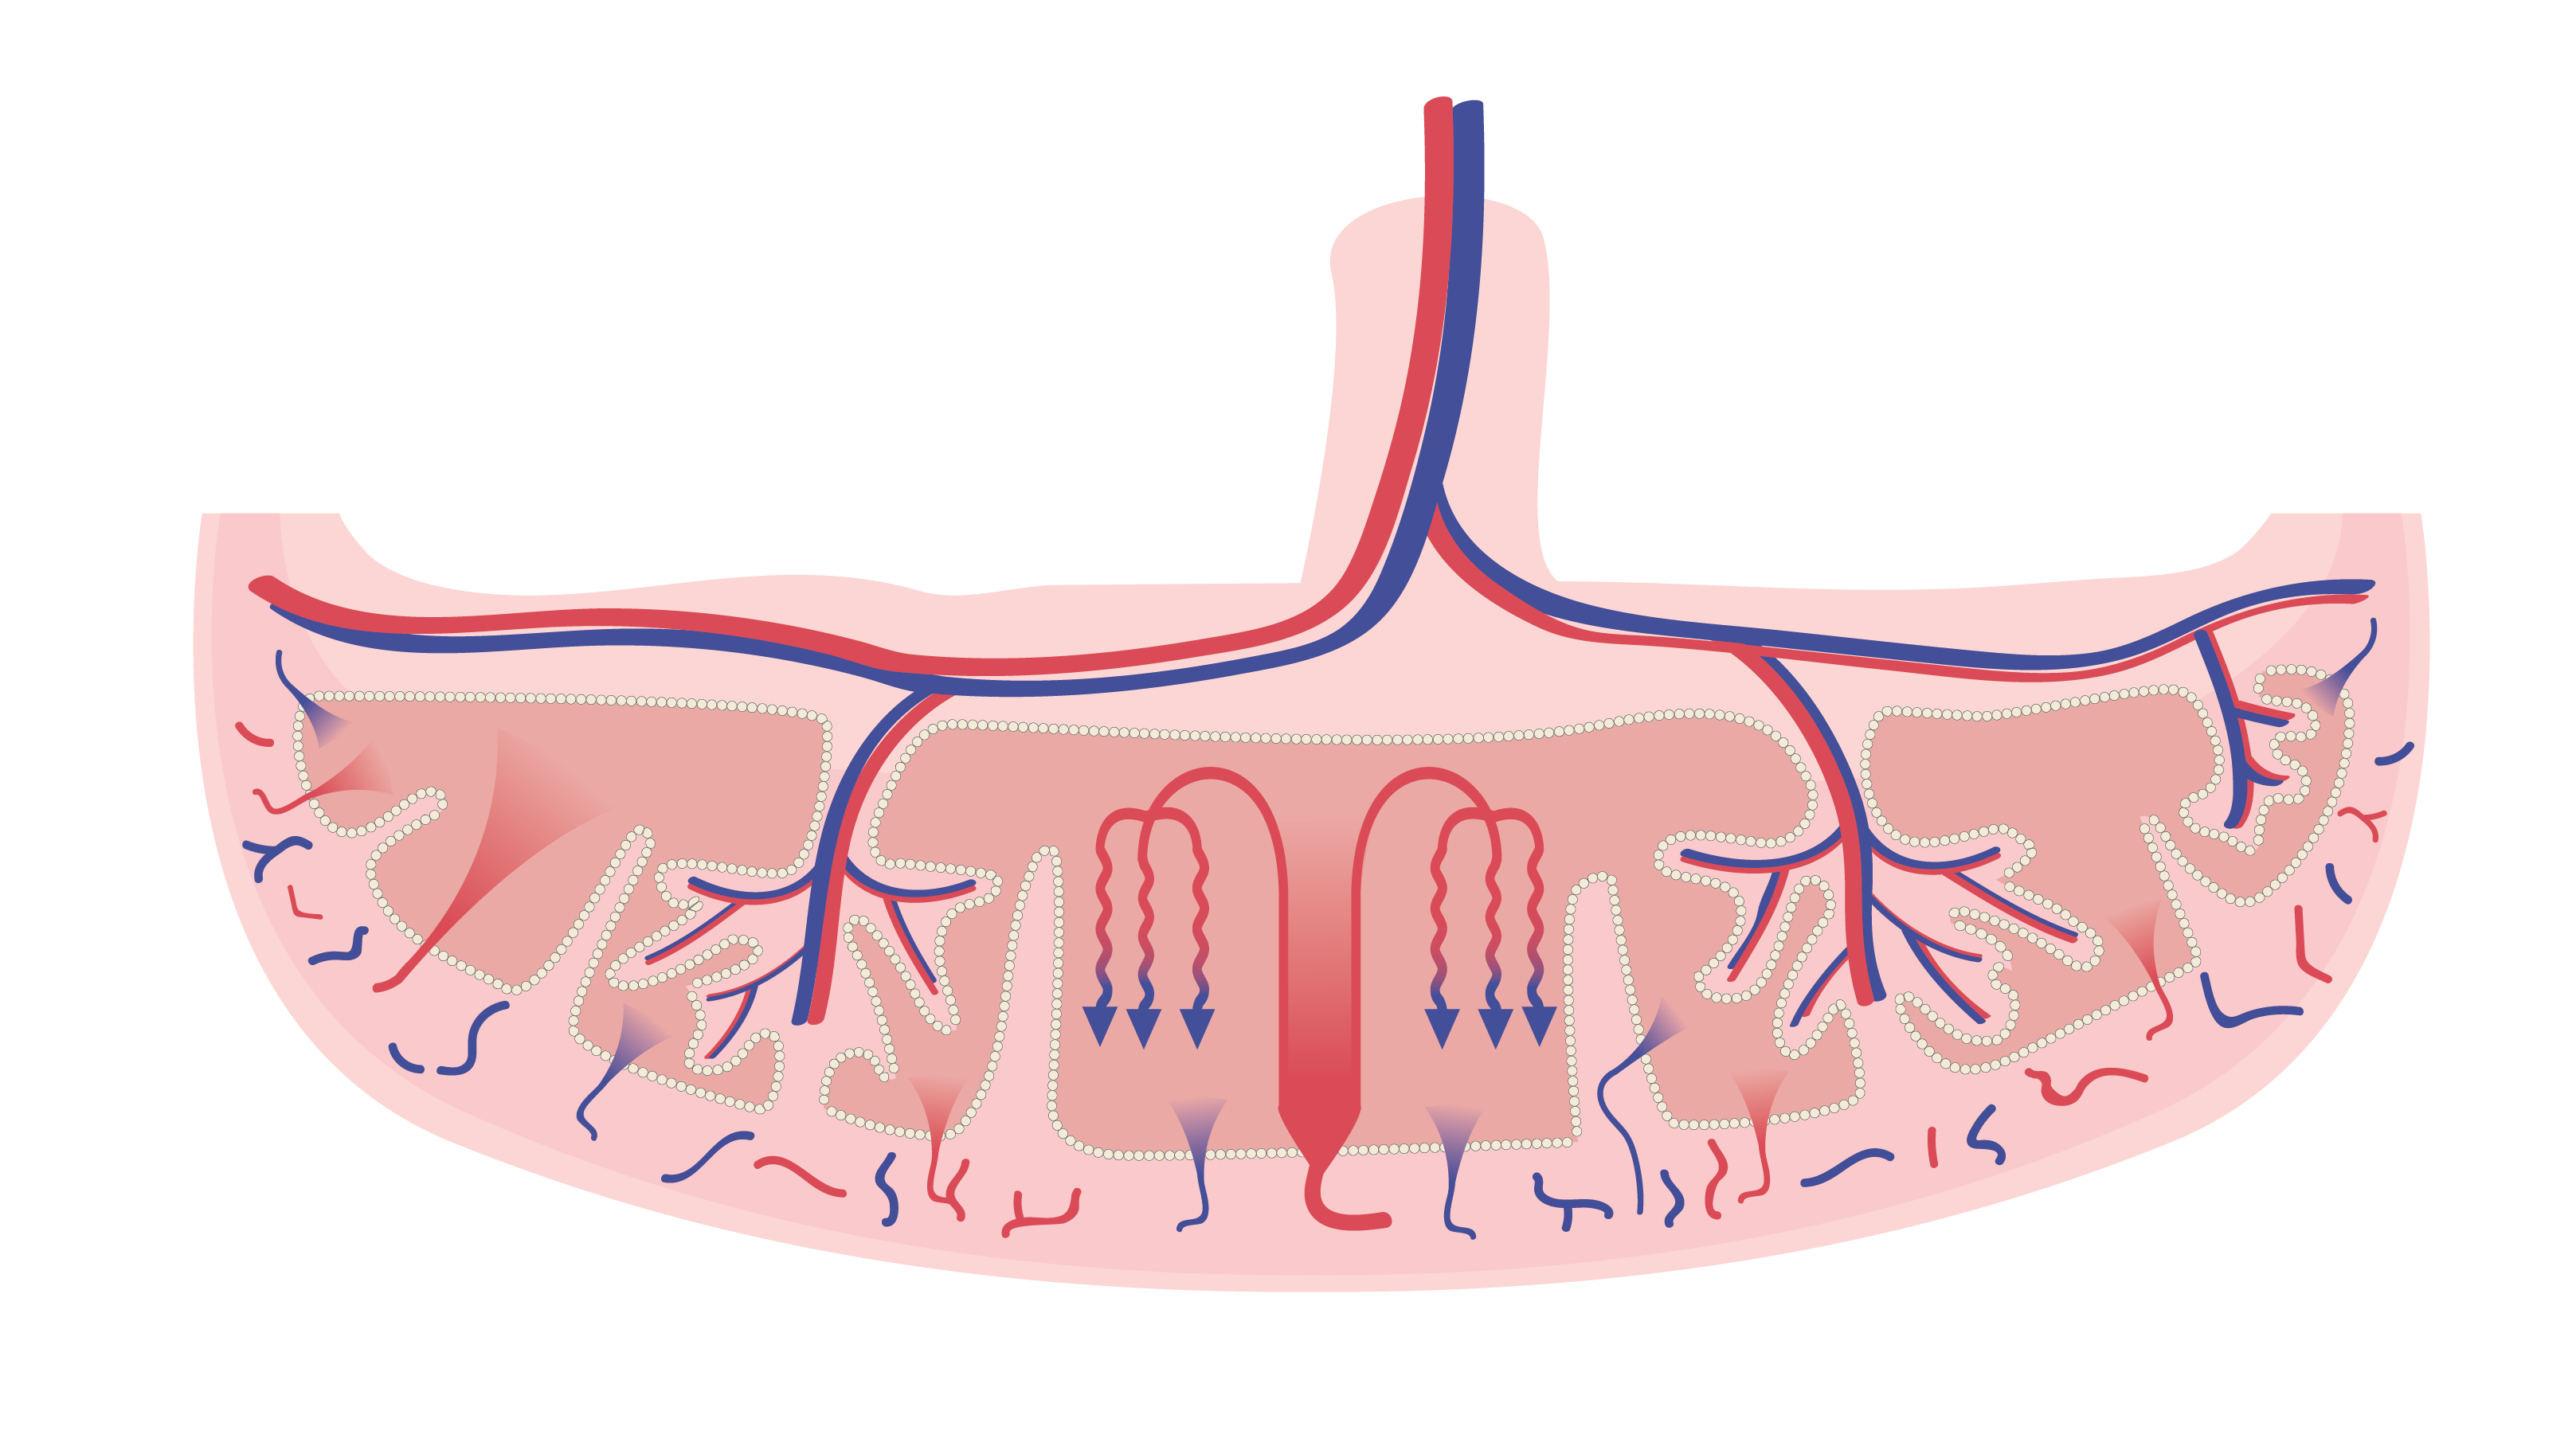
\includegraphics[width=399.29pt,height=225.45pt]{diagrams/placenta-geometry-diagrams/placenta-cartoon-2024.png}};
%Straight Lines [id:da3701239304155397] 
\draw [color={rgb, 255:red, 71; green, 153; blue, 84 }  ,draw opacity=1 ][line width=1.5]    (438,136.13) -- (69.29,136.13) ;
\draw [shift={(65.29,136.13)}, rotate = 360] [fill={rgb, 255:red, 71; green, 153; blue, 84 }  ,fill opacity=1 ][line width=0.08]  [draw opacity=0] (11.61,-5.58) -- (0,0) -- (11.61,5.58) -- cycle    ;
\draw [shift={(442,136.13)}, rotate = 180] [fill={rgb, 255:red, 71; green, 153; blue, 84 }  ,fill opacity=1 ][line width=0.08]  [draw opacity=0] (11.61,-5.58) -- (0,0) -- (11.61,5.58) -- cycle    ;
%Shape: Arc [id:dp7839630490555429] 
\draw  [draw opacity=0][line width=1.5]  (487.26,230.95) .. controls (487.54,232.37) and (487.68,233.81) .. (487.68,235.27) .. controls (487.68,274.09) and (385.83,305.56) .. (260.18,305.56) .. controls (134.53,305.56) and (32.67,274.09) .. (32.67,235.27) -- (260.18,235.27) -- cycle ; \draw [color={rgb, 255:red, 71; green, 153; blue, 84 }  ,draw opacity=1 ][line width=1.5]    (487.68,234.94) .. controls (487.68,235.05) and (487.68,235.16) .. (487.68,235.27) .. controls (487.68,274.09) and (385.83,305.56) .. (260.18,305.56) .. controls (138.3,305.56) and (38.81,275.95) .. (32.95,238.74) ; \draw [shift={(32.67,235.27)}, rotate = 84.01] [fill={rgb, 255:red, 71; green, 153; blue, 84 }  ,fill opacity=1 ][line width=0.08]  [draw opacity=0] (11.61,-5.58) -- (0,0) -- (11.61,5.58) -- cycle    ; \draw [shift={(487.26,230.95)}, rotate = 94.26] [fill={rgb, 255:red, 71; green, 153; blue, 84 }  ,fill opacity=1 ][line width=0.08]  [draw opacity=0] (11.61,-5.58) -- (0,0) -- (11.61,5.58) -- cycle    ;
%Straight Lines [id:da8876380274555917] 
\draw [line width=1.5]    (181.85,82.47) -- (251.5,82.47) ;
\draw [shift={(255.5,82.47)}, rotate = 180] [fill={rgb, 255:red, 0; green, 0; blue, 0 }  ][line width=0.08]  [draw opacity=0] (11.61,-5.58) -- (0,0) -- (11.61,5.58) -- cycle    ;
%Straight Lines [id:da3261920772723992] 
\draw [line width=1.5]    (386,97.81) -- (334.04,185.37) ;
\draw [shift={(332,188.81)}, rotate = 300.69] [fill={rgb, 255:red, 0; green, 0; blue, 0 }  ][line width=0.08]  [draw opacity=0] (11.61,-5.58) -- (0,0) -- (11.61,5.58) -- cycle    ;
%Straight Lines [id:da23004860167795904] 
\draw [color={rgb, 255:red, 124; green, 71; blue, 153 }  ,draw opacity=1 ][line width=1.5]    (421,310.31) -- (376.68,240.74) ;
\draw [shift={(374.53,237.37)}, rotate = 57.5] [fill={rgb, 255:red, 124; green, 71; blue, 153 }  ,fill opacity=1 ][line width=0.08]  [draw opacity=0] (11.61,-5.58) -- (0,0) -- (11.61,5.58) -- cycle    ;
%Straight Lines [id:da26234807553589] 
\draw [color={rgb, 255:red, 218; green, 75; blue, 87 }  ,draw opacity=1 ][line width=1.5]    (260.68,314.42) -- (260.68,290.32) ;
\draw [shift={(260.68,286.32)}, rotate = 90] [fill={rgb, 255:red, 218; green, 75; blue, 87 }  ,fill opacity=1 ][line width=0.08]  [draw opacity=0] (11.61,-5.58) -- (0,0) -- (11.61,5.58) -- cycle    ;
%Straight Lines [id:da659245707576972] 
\draw [color={rgb, 255:red, 71; green, 85; blue, 153 }  ,draw opacity=1 ][line width=1.5]    (353.5,344.31) -- (326.23,255.23) ;
\draw [shift={(325.05,251.4)}, rotate = 72.98] [fill={rgb, 255:red, 71; green, 85; blue, 153 }  ,fill opacity=1 ][line width=0.08]  [draw opacity=0] (11.61,-5.58) -- (0,0) -- (11.61,5.58) -- cycle    ;
%Straight Lines [id:da0549441454891868] 
\draw [color={rgb, 255:red, 248; green, 140; blue, 147 }  ,draw opacity=1 ][line width=1.5]    (177,344.81) -- (195.28,263.52) ;
\draw [shift={(196.15,259.62)}, rotate = 102.67] [fill={rgb, 255:red, 248; green, 140; blue, 147 }  ,fill opacity=1 ][line width=0.08]  [draw opacity=0] (11.61,-5.58) -- (0,0) -- (11.61,5.58) -- cycle    ;
%Straight Lines [id:da750105190473205] 
\draw [color={rgb, 255:red, 71; green, 85; blue, 153 }  ,draw opacity=1 ][line width=1.5]    (454,121.81) -- (466.77,161.26) ;
\draw [shift={(468,165.06)}, rotate = 252.06] [fill={rgb, 255:red, 71; green, 85; blue, 153 }  ,fill opacity=1 ][line width=0.08]  [draw opacity=0] (11.61,-5.58) -- (0,0) -- (11.61,5.58) -- cycle    ;
%Image [id:dp6947304444659705] 
\draw (285.83,93.75) node  {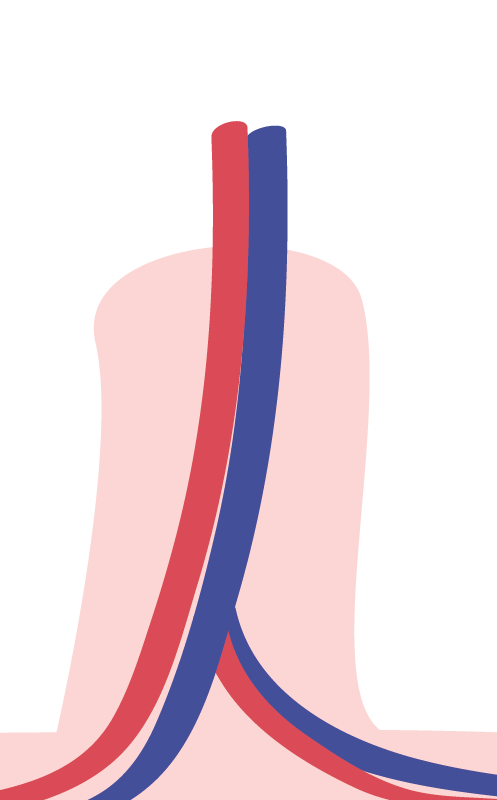
\includegraphics[width=61.5pt,height=98.99pt]{diagrams/placenta-geometry-diagrams/placenta-cartoon-2024_uc.png}};
%Straight Lines [id:da1217993864688609] 
\draw [color={rgb, 255:red, 71; green, 85; blue, 153 }  ,draw opacity=1 ][line width=1.5]    (113.55,313.31) -- (113.55,262.4) ;
\draw [shift={(113.55,258.4)}, rotate = 90] [fill={rgb, 255:red, 71; green, 85; blue, 153 }  ,fill opacity=1 ][line width=0.08]  [draw opacity=0] (11.61,-5.58) -- (0,0) -- (11.61,5.58) -- cycle    ;

% Text Node
\draw (180.89,82) node [anchor=east] [inner sep=0.75pt]   [align=left] {Umbilical cord};
% Text Node
\draw (167.71,128.99) node [anchor=south] [inner sep=0.75pt]  [color={rgb, 255:red, 71; green, 153; blue, 84 }  ,opacity=1 ] [align=left] {Chorionic plate};
% Text Node
\draw (386,94.81) node [anchor=south] [inner sep=0.75pt]   [align=left] {Intervillous space (IVS)};
% Text Node
\draw (421,313.31) node [anchor=north] [inner sep=0.75pt]  [color={rgb, 255:red, 124; green, 71; blue, 153 }  ,opacity=1 ] [align=left] {Villous tree};
% Text Node
\draw (260.68,316.83) node [anchor=north] [inner sep=0.75pt]  [color={rgb, 255:red, 218; green, 75; blue, 87 }  ,opacity=1 ] [align=left] {Spiral artery};
% Text Node
\draw (64.67,279.61) node [anchor=north] [inner sep=0.75pt]  [color={rgb, 255:red, 71; green, 153; blue, 84 }  ,opacity=1 ,rotate=-24.27] [align=left] {Basal plate};
% Text Node
\draw (177,347.81) node [anchor=north] [inner sep=0.75pt]  [color={rgb, 255:red, 248; green, 140; blue, 147 }  ,opacity=1 ] [align=left] {Septal wall};
% Text Node
\draw (454,118.81) node [anchor=south] [inner sep=0.75pt]  [color={rgb, 255:red, 71; green, 85; blue, 153 }  ,opacity=1 ] [align=left] {Marginal sinus vein};
% Text Node
\draw (353.5,347.31) node [anchor=north] [inner sep=0.75pt]  [color={rgb, 255:red, 71; green, 85; blue, 153 }  ,opacity=1 ] [align=left] {Septal wall vein};
% Text Node
\draw (113.55,316.31) node [anchor=north] [inner sep=0.75pt]  [color={rgb, 255:red, 71; green, 85; blue, 153 }  ,opacity=1 ] [align=left] {Basal plate vein};



\end{tikzpicture}
}
                \caption{}
                \label{fig:placenta:cartoon}
            \end{subfigure}
            \caption{(a) Annotated picture provided via private communications with Lopa Leach\protect\footnote{\href{mailto:lopa.leach@nottingham.ac.uk}{lopa.leach@nottingham.ac.uk}} and Dimitrios Amanitis\protect\footnote{\href{mailto:dimitrios.amanitis1@nottingham.ac.uk}{dimitrios.amanitis1@nottingham.ac.uk}}. Picture of the basal plate of a human placenta, with grooves showing visible septal walls. Coloured lines segment the placenta into 5 lobes, with white `L's indicating locations of individual lobules. (b) Modified diagram from \cite{dellschaftHaemodynamicsHumanPlacenta2020}, showing how blood moves through the placenta. The chorionic plate is shown towards the top of the picture, and the basal plate is at the bottom. Septal walls separate individual placentones. Maternal blood enters the placenta via the spiral arteries before percolating through the IVS and exiting through one of three types of vein: basal plate, septal wall, or marginal sinus. Fetal blood enters via the umbilical cord, flows through fetal vessels that cross the chorionic plate, before flowing through the villous trees, and finally returning to the umbilical cord.}
            \label{fig:placenta}
        \end{figure}

        % Development of the placenta throughout gestation.
        The placenta is an organ that develops through gestation, undergoing many structural changes from its initial development to delivery \cite{clarkComputationalModelingInteractions2021}, which complicates placental study. For example, ultrasound measurements indicate placental thickness measured from the umbilical cord insertion site increases almost three-fold between the first and third trimesters (first 14 weeks and after 27 weeks of pregnancy, respectively), increasing from \qty{12.90}{\milli\metre} to \qty{34.67}{\milli\metre} \cite{banikPlacentalThicknessMeasurement2022}. As well as the placenta overall increasing in size, other structural components separately undergo changes. For example, so-called `trophoblast plugs' are present only from approximately 5 weeks of gestation, where cells partially block the spiral artery and promote remodelling (widening) \cite{jamesTrophoblastPlugsImpact2018}. Another example is the villous tree, which matures during gestation to become more specialised for diffusional exchange \cite{hempstockIntralobularDifferencesAntioxidant2003}. This thesis will consider only at-term placentas.

        % Villous tree.
        The exchange of several solutes, including oxygen, takes place through the villous tree, which has a huge surface area  --- approximately $\qty{10}{\metre^2}$, or roughly $10\%$ of the surface area of an adult human's lungs \cite{clarkComplexitiesHumanPlacenta2023}. Efficient exchange often requires maternal blood to access the whole of the villous tree (i.e., areas far from the basal plate), in order to maximise possible uptake area. Figure \ref{fig:hempstock2003} shows how blood enters through spiral arteries, moves through the central cavity (CC), percolates through increasingly mature villous tree material, and then finally exits through one of several veins --- including septal wall veins, marginal sinuses, and other veins located outside the originating placentone by passing over septal walls; naturally, the oxygen concentration in the blood reduces as it passes through the villous tree due to oxygen uptake. It has been postulated that villous density close to spiral arteries must decrease during gestation, in order to account for so-called `mega-jets' that permit deep penetration of nutrient-rich blood \cite{saghianAssociationPlacentalJets2017}. \citeauthor{hempstockIntralobularDifferencesAntioxidant2003} \cite{hempstockIntralobularDifferencesAntioxidant2003} explain that villi nearer to the central cavity are of a larger diameter, and are less specialised for diffusional exchange than their counterparts in the periphery; it is therefore advantageous for high oxygen concentration blood to reach peripheral villi.

        \begin{figure}
            \centering
            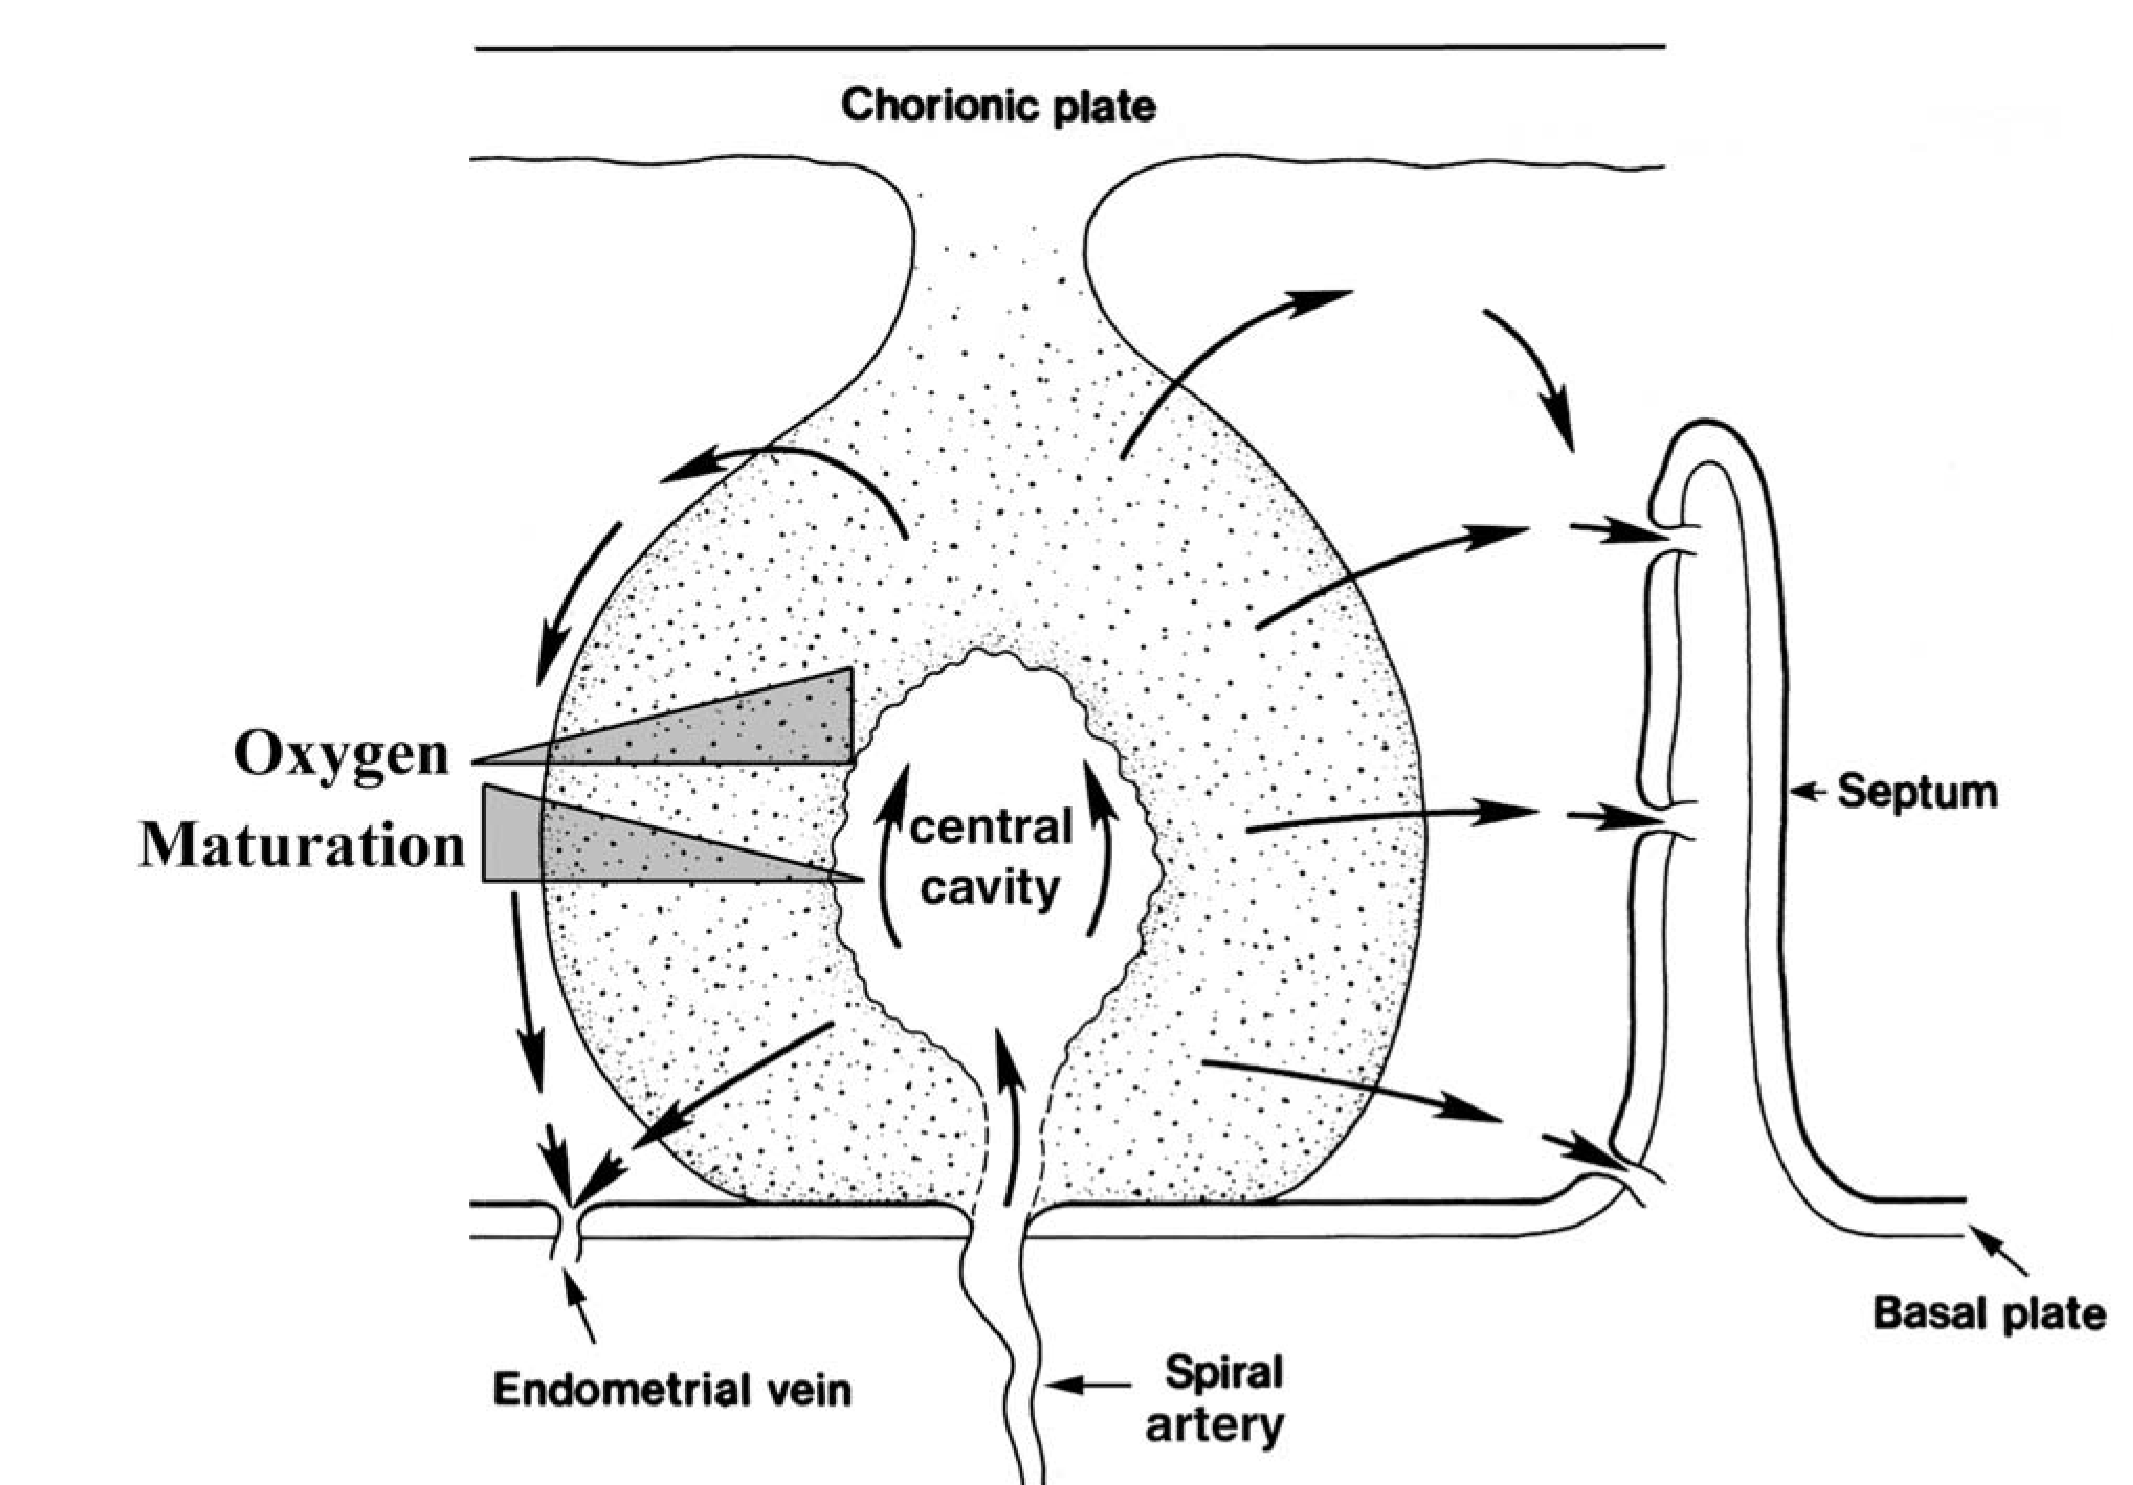
\includegraphics[width=0.6\textwidth]{diagrams/other-paper-figures/hempstock2003.png}
            \caption{Reproduced Figure from \cite{hempstockIntralobularDifferencesAntioxidant2003} showing a single placentone containing a villous tree. The triangles on the left show that outward from the central cavity there is an increasing maturation of villi and a decreasing concentration of blood oxygen.}
            \label{fig:hempstock2003}
        \end{figure}

        % Placental diseases.
        Nutrient delivery is essential for normal fetal growth, with poor delivery of nutrients often linked to pregnancy complications such as stillbirth. A complication of disease study is that some placental diseases are specific to humans \cite{clarkComplexitiesHumanPlacenta2023}, due to radical structural variations between mammalian placentas \cite{laundonPlacentalEvolutionThreedimensional2024}. Pre-eclampsia (PE), for example, is a complex, multisystem disease that is unique to humans, characterised by sudden-onset hypertension \cite{burtonRheologicalPhysiologicalConsequences2009,dimitriadisPreeclampsia2023}. Fetal growth restriction (FGR) is another placental disease that is often associated with stillbirth \cite{smithStillbirth2007}, and is defined as the failure of the fetus to achieve its genetically-determined growth potential \cite{resnikIntrauterineGrowthRestriction2002}, with FGR placentas on average half of the size of normal placentas \cite{sunPlacentaFetalGrowth2020}. PE and FGR are both generally considered to be associated with structural defects in the placenta, leading to impaired nutrient delivery and complications for both the fetus and mother, particularly when spiral arteries fail to widen upon entering the IVS \cite{burtonPathophysiologyPlacentalderivedFetal2018,dellschaftHaemodynamicsHumanPlacenta2020}. In healthy placentas, spiral arteries widen from \qty{0.5}{\milli\metre} to \qtyrange{2}{3}{\milli\metre}, allowing upstream flow to slow from $\qty{1}{\metre\per\second}$ to $\qty{0.1}{\metre\per\second}$; however, in diseased cases, the failure to widen can result in flow at $\qty{1}{\metre\per\second}$ to directly enter the placenta \cite{burtonRheologicalPhysiologicalConsequences2009}. Whilst an increase in flow speed encourages deeper penetration of blood, speeds that are too high will damage villous tree structures, creating an overall smaller uptake area, and reduce blood transit times such that blood leaves the placenta with higher-than-usual oxygen concentrations \cite{burtonRheologicalPhysiologicalConsequences2009}. Understanding which structural changes happen in disease, and the extent to which they impair blood flow and nutrient delivery, may ultimately prove crucial for clinicians looking to treat these diseases. Another source of nutrient delivery impairment has been suggested to be due to whether mothers choose to sleep on their back or on their side; \citeauthor{couperEffectsMaternalPosition2021} \cite{couperEffectsMaternalPosition2021} report that maternal flow rates lower by $27\%$ when mothers are on their backs, as well as a $11.2\%$ decrease in delivery of oxygen to the fetus. This phenomenon occurs even in healthy late-gestation pregnancies, which could be in part an explanation for late-gestation stillbirths. 

        % Speed of flow.
        The work of \citeauthor{burtonRheologicalPhysiologicalConsequences2009} \cite{burtonRheologicalPhysiologicalConsequences2009} and \citeauthor{rothDynamicModelingUteroplacental2017} \cite{rothDynamicModelingUteroplacental2017} focusses on the effects of high flow speed from spiral arteries and the association with diseases such as FGR and PE, and reported the presence of vortices and turbulence in areas surrounding the artery. Even in healthy pregnancies, the speed of flow in the placenta varies greatly from the basal plate to the sub-chorionic space (the region below the chorionic plate, see Figure \ref{fig:placenta:cartoon}). \citeauthor{dellschaftHaemodynamicsHumanPlacenta2020} \cite{dellschaftHaemodynamicsHumanPlacenta2020} gathered data on the speed in the placenta using MRI, and categorised regions of fast flow (flow faster than $\qty{1e-3}{\metre\per\second}$) and slow flow (flow slower than $\qty{5e-4}{\metre\per\second}$), finding that the faster regions were predominantly concentrated on the basal plate. Additionally, they found that there was a distinct difference in the average speed found in the IVS between healthy (\qty{4e-4}{\metre\per\second}) and diseased (\qty{7e-4}{\metre\per\second}) placentas \cite{dellschaftHaemodynamicsHumanPlacenta2020}. 

         % Different types of contractions.
        In addition to dynamics which could arise directly from maternal and fetal blood flow, there are several other forms of movement in the placenta, such as contractions of the villous tree or contractions of the entire uterus; several authors have documented the properties of such phenomena since as early as 1963 \cite{krantzContractilePropertiesSmooth1963,farleyContractilePropertiesHuman2004,lecarpentierUltraslowMyosinMolecular2014,togashiSustainedUterineContractions1993}. However, the newly documented `utero-placental pump' phenomenon is a contraction involving only the placenta \cite{dellschaftHaemodynamicsHumanPlacenta2020}. \citeauthor{dellschaftHaemodynamicsHumanPlacenta2020} \cite{dellschaftHaemodynamicsHumanPlacenta2020} report that it has been found experimentally that placental volume can reduce by up to 40\% in these `utero-placental pump' contractions over a 10-minute period, resulting in a periodic ejection of blood from the IVS. 

        % Perfusion experiments.
        Delivered placentas, whilst generally readily-available after birth, undergo significant structural changes outside the uterus \cite{lecarpentierComputationalFluidDynamic2016}, rendering ex vivo experiments of limited use. One way of overcoming the deflation issue is to perform perfusion experiments soon after delivery, where a placentone is identified in a freshly delivered placenta, and both the maternal and fetal blood supplies are catheterised \cite{schneiderModifiedDoublecircuitVitro1984,lewisPlacentalPerfusionMathematical2020}; these have then been coupled with mathematical models, giving a well-controlled system in which to test parameters and gain physiological understanding \cite{lewisPlacentalPerfusionMathematical2020}. In the case where placentas fail entirely, artificial placentas have been developed since as early as the 1950s with variable success; however, important progress towards the ultimate goal of a functioning artificial human placenta has been made through important contributions to placental research throughout the 2010s \cite{tunDifferencesPlacentalCapillary2019,saghianAssociationPlacentalJets2017,katoVillousTreeModel2017,serovOptimalVilliDensity2015,serovRoleMorphologyMathematical2016,lecarpentierComputationalFluidDynamic2016,clarkMultiscaleModellingFeto2015,chernyavskyTransportPlacentaHomogenizing2011,chernyavskyMathematicalModelIntervillous2010,burtonRheologicalPhysiologicalConsequences2009,lewisPlacentalPerfusionMathematical2020}.
        
        % Digital twins.
        Mathematical modelling is a powerful tool in developing understanding of behaviour in complex systems, such as the placenta and other organs. Digital twins are regarded as the gold standard of organ modelling, where simulations directly model a specific real-world organ. Sufficiently developed digital twins of the placenta would allow clinicians to study disease and the effects of medical intervention in a risk-free environment. Whilst there are currently no such models of the entire placenta, mathematical modelling of the heart has made use of patient-specific geometries \cite{taoDigitalTwinModeling2022}, with projects such as iHEART contributing to collective understanding of the organ \cite{zingaroComprehensiveMathematicalModel2023}. Upon the path leading to digital twins of the human placenta lies several issues that must first be tackled by the modelling community; \citeauthor{jensenBloodFlowTransport2019} \cite{jensenBloodFlowTransport2019} detail the important issues as modelling deformability of villous trees, impact from the external environment, 3D morphology at a statistical level, development of the placenta from early pregnancy, transport of multiple substances, and understanding structural variations across placental mammalian species.
        
    \section{Flow and transport in the placenta}
        % Fetal/maternal flow in isolation.
        Most current mathematical models consider either the fetal or maternal blood flow in isolation. This thesis focusses solely on modelling the maternal blood, but we now give a brief overview of fetal modelling approaches.

        % Fetal modelling.
        \citeauthor{zhangRecastingCurrentKnowledge2023} \cite{zhangRecastingCurrentKnowledge2023} highlight the importance of computational models in the study of fetal blood flow.
        The behaviour of fetal blood is often directly linked to the structure of the villous tree, leading many recent studies to use anatomical images to study fetal flow behaviour on the scale of individual villous tree `leaves' \cite{erlichPhysicalGeometricDeterminants2019,erlichQuantifyingImpactTissue2019,pearceImageBasedModelingBlood2016,plitmanmayoThreedimensionalModelingHuman2016}. \citeauthor{clarkMultiscaleModellingFeto2015} \cite{clarkMultiscaleModellingFeto2015} were instead able to create an anatomically based geometric model of the entire fetal villous tree, and used a simple flow model to study how fetal blood was affected by changes to the structure of the tree. The umbilical cord carries the fetal blood to and from the placenta; \citeauthor{kasiteropoulouComputationalFluidDynamics2020} \cite{kasiteropoulouComputationalFluidDynamics2020} studied the structure of the umbilical cord and how this impacts heat exchange, finding that the helicity of the cord plays a vital role in fetal thermoregulation.

        % Types of maternal modelling.
        In the existing literature, there are generally two approaches to modelling maternal blood flow \cite{jensenBloodFlowTransport2019}. Firstly, there are pore-scale (or micro-scale) models, where `pore' refers to the volume between villous tree branches; for example, \citeauthor{lecarpentierComputationalFluidDynamic2016} \cite{lecarpentierComputationalFluidDynamic2016} take 2D anatomical images of the villous trees and use the Navier-Stokes equations to model blood flow through the pores, although the method of imaging was not reported. An inherent issue with this 2D approach is that tree material can form impenetrable barriers in the plane, a constraint that 3D flow models may overcome. \citeauthor{serovOptimalVilliDensity2015} \cite{serovOptimalVilliDensity2015} used the micro-scale approach to simulate flow through a `stream-tube placenta model' and measured oxygen uptaken by the villous tree, ultimately finding an optimal villous density of approximately $0.47$ maximises oxygen uptake, which is consistent with previous experimental measurements. Secondly, there are tree-scale (or macro-scale) models, which model flow through gaps in the tree branches as a porous medium via, for example, a Darcy-type description \cite{lecarpentierComputationalFluidDynamic2016,chernyavskyMathematicalModelIntervillous2010,erianMaternalPlacentalBlood1977}; this involves creating a resistance to flow, which can be described by a permeability (equivalently hydraulic conductivity) $k$, for which the size of $k$ is inversely proportional to the effective flow resistance.

        % Majority of the Darcy-type maternal modelling.
        In \citeyear{erianMaternalPlacentalBlood1977}, \citeauthor{erianMaternalPlacentalBlood1977} \cite{erianMaternalPlacentalBlood1977} were the first to model maternal placenta flow computationally. They modelled the placentone as a square, through which blood flowed according to Darcy's law, with a permeability field that varied with position, accounting in a simple way for a less-permeable central cavity region. This porous medium approach has been adopted more recently by \citeauthor{chernyavskyMathematicalModelIntervillous2010} \cite{chernyavskyMathematicalModelIntervillous2010} where they derive analytical expressions for the blood flow field, under the assumption of Darcy flow in a 3D hemispherical domain representing a single placentone. \citeauthor{lecarpentierComputationalFluidDynamic2016} \cite{lecarpentierComputationalFluidDynamic2016} computationally modelled flow through a single 2D placentone, from which they were able to inform wall shear stress (WSS) villous tree measurements on several small areas cut out from the domain. This work provides valuable insight into the stresses experienced by cells in the villous tree, as it is believed that diseases such as PE may be attributed to damage to the villous tree caused by high-speed flow \cite{burtonRheologicalPhysiologicalConsequences2009}.

        % Central cavity.
        The central cavity is a villous-free region above the spiral artery mouth, thought to form among the villous tree material due to stresses from incoming maternal blood flow \cite{burtonRheologicalPhysiologicalConsequences2009,saghianAssociationPlacentalJets2017}. This region provides a lower resistance to flow, allowing incoming high-speed flow to penetrate deeper into the placenta before entering the IVS. In the context of the placenta, regions of high-speed flow (faster than $\qty{0.1}{\metre\per\second}$) are referred to as `jets' \cite{saghianAssociationPlacentalJets2017}. Ultrasound imaging have found so-called `mega-jets', which are jets longer than half of the placental thickness, and are components of a normal pregnancy \cite{collinsDevelopmentalChangesSpiral2012}. \citeauthor{saghianAssociationPlacentalJets2017} \cite{saghianAssociationPlacentalJets2017} modelled flow entering the IVS throughout gestation, finding that the presence of mega-jets requires regions of less dense villous tree, such as the central cavity. 
        
        % Advancements.
        Some authors employ a hybrid between the micro- and macro-scale approaches, using micro-scale simulations to determine values of local permeability, which then informs the macro-scale dynamics through a spatially varying permeability field \cite{lecarpentierComputationalFluidDynamic2016,linMultiscaleModelPlacental2016}. Some authors who use macro-scale models make further modelling enhancements such as varying the permeability throughout the domain \cite{lecarpentierComputationalFluidDynamic2016,erianMaternalPlacentalBlood1977}, or modelling the effect of artery widening before the maternal blood enters the IVS, to study what effect this has on fetal development \cite{burtonRheologicalPhysiologicalConsequences2009,rothDynamicModelingUteroplacental2017,saghianAssociationPlacentalJets2017}. Whilst most of the mathematical placental literature studies third trimester placentas (usually regarded as `fully developed' or `at term'), some authors have investigated the placenta throughout its development. For example, \citeauthor{jamesTrophoblastPlugsImpact2018} \cite{jamesTrophoblastPlugsImpact2018} computationally investigated the effect of trophoblast plugs, with their work suggesting that trophoblast plugs play an important role in rate-limiting flow to the placenta, and that malformation of these plugs can lead to diseased placentas. Little is known about the rheology of blood in the IVS when compared to blood rheology in narrow capillaries, which have been well-characterised experimentally, and instead authors model maternal blood flow in the IVS as incompressible \cite{chernyavskyMathematicalModelIntervillous2010}.

        % Transport models.
        Exchange from mother to fetus is also an important aspect to study, for which the flow of blood can be regarded as a vehicle in which to transport oxygen, nutrients, and waste products. Some authors have modelled transport using a reaction-advection equation for oxygen or nutrient concentration \cite{perazzoloModellingEffectIntervillous2017,perazzoloModellingNutrientTransfer2016,chernyavskyMathematicalModelIntervillous2010}, whilst others have supplemented the reaction-advection equation using Henry's law, which additionally describes enhancement to advection due to oxygen's affinity for haemoglobin \cite{serovOptimalVilliDensity2015,erlichPhysicalGeometricDeterminants2019,pearceImageBasedModelingBlood2016,meklerImpactTissuePorosity2022,serovOptimalVilliDensity2015,pearceImageBasedModelingBlood2016}.

        % Contractions.
        Given that the placenta lacks stiff supporting inner structures, a poroelastic description is likely appropriate \cite{jensenBloodFlowTransport2019}. Moreover, throughout gestation, contractions of the placenta and surrounding uterus have been widely reported \cite{dellschaftHaemodynamicsHumanPlacenta2020,togashiSustainedUterineContractions1993,farleyContractilePropertiesHuman2004}. However, as far as we are aware, there is currently only one paper that presents a mathematical model that describes contractions. \citeauthor{katoVillousTreeModel2017} \cite{katoVillousTreeModel2017} focussed on the effect of actively contracting villous trees, finding the contractions to be useful for both the fetal and maternal blood circulations due to resulting displacements. Whilst the recently-discovered utero-placental pump is yet to be mathematically modelled, it is thought that these contractions may be related to the previous reports of contracting villous trees \cite{dellschaftHaemodynamicsHumanPlacenta2020}.

        % Coupled models.
        Little work has been undertaken on fully-coupled transport models describing both maternal and fetal flow simultaneously, especially at the organ-scale. The first coupled transport paper we are aware of is from 1973, where \citeauthor{hillMathematicalModelCarbon1973} \cite{hillMathematicalModelCarbon1973} used a simple compartmental model to describe the transport of oxygen and carbon dioxide between maternal and fetal blood, which allowed the authors to investigate the relationship between Haldane and Bohr effects and transport. More recently, the use of mathematical models in combination with perfusion experiments is summarised by \citeauthor{lewisPlacentalPerfusionMathematical2020} \cite{lewisPlacentalPerfusionMathematical2020}, where the authors highlight several studies that have used compartmental models --- which describes how solutes may pass between mother, placenta, and fetus --- in order to study the bidirectional transport behaviour of various solutes in artificial perfusion experiments \cite{stirratTransferMetabolismCortisol2018,perazzoloInfluencePlacentalMetabolism2017,lofthouseComputationalModellingParacellular2023,hirschmuglPlacentalMobilizationFree2021}. Other related studies have modelled solute passing from maternal flow to the fetal capillaries, but for simplicity neglect the fetal flow itself \cite{perazzoloModellingEffectIntervillous2017}.

        % Structural variations.
        One of the most significant difficulties of placental study is that structural variability is not well understood \cite{jensenBloodFlowTransport2019}. To illustrate this, \citeauthor{benirschkePathologyHumanPlacenta2012} \cite{benirschkePathologyHumanPlacenta2012} took two vastly different estimates of the number of spiral arteries from previous studies, where one author estimated $263$, whilst another estimated just $25$; the disparity here is likely due to difficulties in identifying the arteries, and also due to functional changes to the arteries during development \cite{benirschkePathologyHumanPlacenta2012}. Contrasting estimates can also be found for other structural features, such as the number and position of veins \cite{chernyavskyMathematicalModelIntervillous2010,boydHumanPlacenta1970}, and the number of placentones \cite{benirschkePathologyHumanPlacenta2012,kaufmannPlacentalVascularizationBlood1988,serovOptimalVilliDensity2015,boydHumanPlacenta1970}. In the absence of a concrete understanding of many important structural features, several studies have used mathematical models to investigate their impact on placental behaviour. For example, \citeauthor{chernyavskyMathematicalModelIntervillous2010} \cite{chernyavskyMathematicalModelIntervillous2010}, and more recently \citeauthor{meklerImpactTissuePorosity2022} \cite{meklerImpactTissuePorosity2022}, studied how vein placement affects oxygen uptake to the villous tree; they found that veins too close to the artery would exhibit `short-circuiting' behaviour, where flow is very much localised to the region between the arteries and veins, thus limiting oxygen uptake. \citeauthor{chernyavskyMathematicalModelIntervillous2010} \cite{chernyavskyMathematicalModelIntervillous2010} also studied how the height of the villous-free central cavity influences oxygen concentration, finding deeper penetration of oxygen for larger cavity sizes.

        % Standard maternal blood flow model.
        A standard model in the maternal mathematical literature has been to allocate one artery and two veins on the basal plate to a placentone, with mathematical models of maternal blood flow restricted to placentones, and therefore do not consider either septal wall or marginal sinus veins. This is a clear limitation of existing studies as flux of blood between neighbouring placentones, as would be expected in the sub-chorionic space (SCS) \cite{jensenBloodFlowTransport2019}, is necessarily neglected. Furthermore, additional drainage due to septal wall veins and marginal sinus veins have not been considered in flow models, despite reports of their existence in the literature \cite{hempstockIntralobularDifferencesAntioxidant2003,AMANITIS2023e68,nanaevHumanPlacentaEncircled2000}. Although there are several works related to simulations of entire fetal villous trees (e.g., \cite{clarkMultiscaleModellingFeto2015,tunDifferencesPlacentalCapillary2019}), as far as we are aware, there is not any published work that tackles simulations of maternal blood flow on the scale of the entire placenta.
        
        % What we're doing.
        In this thesis, we exclusively use a macro-scale model of maternal blood flow. This approach eliminates the need for fine villous tree meshes, gives the permeability field as a simple function of the spatial coordinates, and avoids challenges that arise with impermeable villous tree structures in 2D. We will also adopt some of the modelling enhancements in the aforementioned references, such as the inclusion of a central cavity and a widening spiral artery. As noted by \citeauthor{jensenBloodFlowTransport2019} in \cite{jensenBloodFlowTransport2019}, the described approaches for maternal haemodynamics are mostly restricted to single placentones; \citeauthor{jensenBloodFlowTransport2019} further note that there is meaningful progress still to be made at the whole-organ level, and with validating models against experimental data. We will therefore solve a macro-scale model on a representative 2D slice of a whole placenta, which as far as we are aware, is a novel contribution of this thesis. This 2D geometry is simpler than an equivalent 3D geometry, but captures the main structural features of the placenta. Our blood flow model will be supplemented with a model of oxygen transport so that we may study oxygen uptake by the fetal villous tree. The thesis will then develop in three separate settings: to investigate how placental structure influences flow and transport; to model MRI scans of placental flow; and to introduce a preliminary model of utero-placental pump.
        
    \section{Models of flow} 
        % Darcy's law.
        Poromechanics more generally describes the behaviour of fluids saturating porous media, where the fluid may be a liquid or a gas, and the structure is often permeable or elastic (e.g., \cite{collisEffectiveEquationsGoverning2017}). The simplest example of steady flow through a porous medium is Darcy's law. For a bounded domain $\Omega \subset \RR^d$, for $d = 2, 3$, Darcy's law is given by
        \begin{equation}
            \frac{\mu}{k} \vec{u} + \vec{\nabla}p = 0,
            \label{eq:darcy-law}
        \end{equation}
        where $\vec{u}$ is the vector velocity field of the fluid, $p$ is the scalar pressure field, $k$ is permeability, and $\mu$ is the dynamic viscosity of the fluid. We have omitted boundary conditions here for ease of presentation.

        % Navier-Stokes.
        The Navier-Stokes equations model time-dependent, viscous, Newtonian (non-porous) fluid flow. The incompressible Navier-Stokes equations are given as: find $\vec{u}, p$ such that
        \begin{subequations}
            \begin{align}
                \begin{split}
                    \rho \pdv{\vec{u}}{t} + \rho (\vec{u} \cdot \vec{\nabla}) \vec{u} - \mu \nabla^2 \vec{u} + \vec{\nabla} p & = \rho \vec{f},
                \end{split}\\
                \begin{split}
                    \vec{\nabla} \cdot \vec{u} & = 0,
                \end{split}%
            \end{align}%
            \label{eq:navier-stokes}%
        \end{subequations}%
        where $\rho$ is the density of the fluid, and $\vec{f}$ is some body force acting on the fluid. One may define the Reynolds number as $\Rey := \frac{\rho U L}{\mu}$, for some appropriate choices of velocity and length scalings ($U$ and $L$, respectively), which describes the ratio between inertial and viscous forces. By assuming that the inertial forces are small compared to viscous forces, the Reynolds number is low (i.e., $\Rey \ll 1$), Equation \eqref{eq:navier-stokes} at leading order reduces to Stokes flow: find $\vec{u}, p$ such that
        \begin{subequations}
            \begin{align}
                \begin{split}
                    - \mu \nabla^2 \vec{u} + \vec{\nabla} p & = \vec{f},
                \end{split}\\
                \begin{split}
                    \vec{\nabla} \cdot \vec{u} & = 0.
                \end{split}
            \end{align}
            \label{eq:stokes-flow}
        \end{subequations}
        
        % Brinkman.
        In \citeyear{brinkmanCalculationViscousForce1949}, \citeauthor{brinkmanCalculationViscousForce1949} \cite{brinkmanCalculationViscousForce1949} introduced a modification of Darcy's law in Equation \eqref{eq:darcy-law}, which we will refer to as the Brinkman equations: find $\vec{u}, p$ such that
        \begin{subequations}
            \begin{align}
                \begin{split}
                    - \Tilde{\mu} \nabla^2 \vec{u} + \frac{\mu}{k} \vec{u} + \vec{\nabla} p & = \vec{0},
                \end{split}\\
                \begin{split}
                    \vec{\nabla} \cdot \vec{u} & = 0,
                \end{split}%
            \end{align}%
            \label{eq:brinkman}%
        \end{subequations}%
        where $\Tilde{\mu}$ is the so-called effective viscosity \cite{nieldConvectionPorousMedia2017}. As well as this equation being second order --- and therefore allowing consistent application of boundary or interface conditions with, say, the Navier-Stokes equations --- \citeauthor{brinkmanCalculationViscousForce1949} remarks that this equation has the advantage of approximating Darcy flow in Equation \eqref{eq:darcy-law} for small values of $k$, and Stokes flow in Equation \eqref{eq:stokes-flow} for high values of $k$. Typically, most authors make the simplification of $\Tilde{\mu} = \mu$ \cite{auriaultDomainValidityBrinkman2009}.

        % Navier-Stokes-Darcy.
        In porous media applications where inertial effects are important, the so-called Navier-Stokes-Darcy (or equivalently Navier-Stokes-Brinkman) equations may be more appropriate. These equations consist of Navier-Stokes equations augmented by an additional Darcy drag term and have previously been used to simulate solid obstacles in a fluid domain or imposing no-slip boundary conditions \cite{angotPenalizationMethodTake1999,fuchsbergerIncorporationObstaclesFluid2022}, and for directly modelling insect flight \cite{engelsFluSINovelParallel2016} and flow involved in matrix acidising \cite{jiaModelingAnalysisCarbonate2021}. The Navier-Stokes-Darcy equations are given by: find $\vec{u}$, $p$ such that
        \begin{subequations}
            \begin{align}
                \begin{split}
                    \rho \pdv{\vec{u}}{t} + \frac{\mu}{k}\vec{u} + \rho (\vec{u} \cdot \vec{\nabla}) \vec{u} - \mu \nabla^2 \vec{u} + \vec{\nabla} p & = \rho \vec{f},
                \end{split}\\
                \begin{split}
                    \vec{\nabla} \cdot \vec{u} & = 0.
                \end{split}%
            \end{align}%
            \label{eq:navier-stokes-darcy}%
        \end{subequations}%
        Other related models include the Brinkman-Forchheimer equations, where the drag is modelled by both a Darcy-type term and a quadratic drag term that scales with $\vec{u}|\vec{u}|$ \cite{hsuThermalDispersionPorous1990,nieldLimitationsBrinkmanForchheimerEquation1991}. The additional Forchheimer term is generally applicable to flow of high Reynolds number ($\Rey > 100$) \cite{nieldConvectionPorousMedia2017}.

        % Poromechanics in the placenta.
        In many porous flow applications, such as those in the placenta, there are regions of `free' flow (often modelled by Stokes flow or the Navier-Stokes equations) and regions of porous flow (often modelled by Darcy's law or the Brinkman equations). The approach adopted in this thesis is to use a single partial differential equation (PDE) on the entire domain that captures effects of both free and porous flow in the appropriate regions.
            
    % Numerical approaches
    \section{Numerical methods}
        % What others have done.
        Finite element methods (FEMs) are one of many choices of numerical methods for approximating solutions to PDEs. FEMs first appeared in work by \citeauthor{courantVariationalMethodsSolution1943} in \citeyear{courantVariationalMethodsSolution1943}, where the author used the idea of minimising a functional using linear approximations over subregions, which is fundamental to the formulation required for deriving a finite element method \cite{courantVariationalMethodsSolution1943}. \citeauthor{cloughFiniteElementMethod1960} in \citeyear{cloughFiniteElementMethod1960} gave the method its name, describing how the methods could be used on models of wing structure flexibility at Boeing \cite{cloughFiniteElementMethod1960}. The initial development of FEMs are also credited by \citeauthor{guptaBriefHistoryBeginning1996} \cite{guptaBriefHistoryBeginning1996} to papers by \citeauthor{argyrisEnergyTheoremsStructural1960} \cite{argyrisEnergyTheoremsStructural1960}, \citeauthor{turnerStiffnessDeflectionAnalysis1956} \cite{turnerStiffnessDeflectionAnalysis1956}, and \citeauthor{zienkiewiczFiniteElementMethod1989} \cite{zienkiewiczFiniteElementMethod1989}. Since the initial work, many different flavours of FEMs have been developed including the very popular continuous Galerkin FEMs (CGFEMs) \cite{ciarletFiniteElementMethod2002}, discontinuous Galerkin FEMs (DGFEMs) which this work exploits \cite{arnoldUnifiedAnalysisDiscontinuous2006}, as well as extended FEMs (XFEMs) \cite{Moes1999AFiniteelementMethodForCrackGrowth}, cut FEMs (CutFEMs) \cite{burmanCutFEMDiscretizingGeometry2015}, and the closely-related virtual element methods (VEMs) \cite{beiraodaveigaBasicPrinciplesVirtual2013} and finite volume methods (FVMs) \cite{moukalledFiniteVolumeMethod2016} --- some of which can be combined to make very powerful methods.

        % Numerical methods in the placenta.
        Whilst some studies of maternal placental flow have derived analytical expressions of flow (e.g., \cite{chernyavskyMathematicalModelIntervillous2010,burtonRheologicalPhysiologicalConsequences2009}), the vast majority of studies cited in this thesis have approximated PDE solutions using one of two software packages: ANSYS Fluent \cite{meklerImpactTissuePorosity2022,saghianAssociationPlacentalJets2017} or COMSOL Multiphysics \cite{lecarpentierComputationalFluidDynamic2016,perazzoloModellingNutrientTransfer2016,perazzoloModellingEffectIntervillous2017}. Whilst the details of the discretisations are not presented in these studies, we can infer that discretisations of spatial derivatives use FVMs in ANSYS Fluent, and either CGFEMs or FVMs in COMSOL Multiphysics.

        % DGFEMs.
        Loosely speaking, DGFEMs are somewhat of a hybrid between classical CGFEMs and FVMs \cite{cangianiHpVersionDiscontinuousGalerkin2017}, the latter being used extensively in computational fluid dynamics (CFD) simulations. \citeauthor{cangianiHpVersionDiscontinuousGalerkin2017} \cite{cangianiHpVersionDiscontinuousGalerkin2017} highlight that DGFEMs are an excellent choice for modelling in many practical settings due to their simple treatment of complicated geometries, stability properties for large parameter variations, and favourable treatment of hyperbolic terms in PDEs. In particular, DGFEMs are highly parallelisable from a computational viewpoint as elements only involve communication across element faces, allowing some computations to take place independently of each other \cite{flahertySoftwareParallelAdaptive2000}.

        % What we do.
        For the numerical simulations undertaken here, we employ DGFEMs as our numerical method of choice. We note that we specifically use the DGFEM symmetric interior penalty method, which is both consistent and stable \cite{arnoldUnifiedAnalysisDiscontinuous2006}. DGFEMs form a natural choice of method for our application due to the inherent complicated placental geometries and fast deceleration of flow as blood enters the placenta.

    % 1.3 MRI and imaging
    \section{Magnetic resonance imaging (MRI)}
        % Introduce point, what one may learn
        % Approaches, modelling, ...
        % Give short description/summary of what George does? Point forward if you really want to keep it there.

        % Overview of MRI.
        Magnetic resonance imaging (MRI) is an imaging technique that uses a strong magnetic field and radio waves to generate images of biological tissue. These images are predominantly used to non-invasively investigate pathology in the human body. This thesis will specifically focus on the modelling of motion-sensitising MRI, where magnetic field pulses are applied in a specific configuration to measure a velocity field (see \cite{bernsteinHandbookMRIPulse2004} for a comprehensive summary of MRI techniques).

        % History.
        \citeauthor{rinck2008short} \cite{rinck2008short} outlines the history of MRI development; MRI originated in \citeyear{blochNuclearInduction1946} from the discovery of nuclear magnetic resonance (NMR) by \citeauthor{blochNuclearInduction1946} \cite{blochNuclearInduction1946} and \citeauthor*{purcellResonanceAbsorptionNuclear1946} \cite{purcellResonanceAbsorptionNuclear1946}, where particles emit electromagnetic signals under strong magnetic fields. The medical applications of NMR were realised by Odeblad, who applied NMR to living cells and excised animal tissue throughout the 1950s and 1960s (e.g., \cite{odebladPreliminaryObservationsProton1955,odebladProtonMagneticResonance1956,odebladFunctionalStructureHuman1968}). In the early 1970s, Lauterbur and Mansfield created techniques that spatially encoded NMR signals, thus permitting NMR imaging (i.e., MRI) for the first time. \citeauthor*{lauterburMagneticResonanceZeugmatography1974} \cite{lauterburMagneticResonanceZeugmatography1974} produced the very first MRI image of a living animal --- a clam --- in \citeyear{lauterburMagneticResonanceZeugmatography1974}, whilst \citeauthor*{mansfieldMedicalImagingNMR1977} \cite{mansfieldMedicalImagingNMR1977} created the first image of in vivo human anatomy --- a finger --- in \citeyear{mansfieldMedicalImagingNMR1977}. Since the 1980s, commercial development of scanners and widespread use in hospitals have made MRI scanners an indispensable technique for non-invasive imaging of pathology in vivo, including the placenta.

        % MRI modelling.
        Nuclear magnetisation is an intrinsic property of particles with an odd number of protons and neutrons. Hydrogen has 1 proton and 1 neutron, and is predominantly used for measurements due to its relative abundance in water and fat in the human body \cite{bushbergEssentialPhysicsMedical2012}. Nuclear magnetisation has both a strength and a direction, and its evolution in particles is described by the Bloch-Torrey equation \cite{bushbergEssentialPhysicsMedical2012,nguyenFiniteElementsMethod2014}. \citeauthor{nguyenFiniteElementsMethod2014} \cite{nguyenFiniteElementsMethod2014} write the Bloch-Torrey equation as: find $M(\vec{r}, t)$ such that 
        \begin{equation}
            \pdv{M(\vec{r}, t)}{t} = -i \gamma (\vec{G} \cdot \vec{r}) M + \vec{\nabla} \cdot (\vec{D} \vec{\nabla} M),
            \label{eq:bloch-torrey}
        \end{equation}
        where $M(\vec{r}, t) \in \CC$ is nuclear magnetisation, $\vec{G}$ is a magnetic gradient (to be introduced in \S\ref{sec:numerical-mri:preliminaries}), $\vec{r}$ is displacement of particles, $t$ is time, $i$ is the imaginary unit, $\gamma$ is the gyromagnetic ratio, and $\vec{D}$ is a molecular diffusion matrix. MRI scanners make use of many non-overlapping cuboidal voxels covering the domain of interest, from which MRI scanners measure the collective nuclear magnetisation of the particles contained in each voxel; this is achieved through the magnetic properties of the hydrogen atom, which is abundant in water and fat \cite{bergerHowDoesIt2002}. Chapter \ref{sec:numerical-mri} will infer MRI signals using Equation \eqref{eq:bloch-torrey}, where we assume $\vec{D} = \vec{0}$ (i.e., the Bloch equation) as so-called pseudo-diffusive effects dominate in studies of blood flow \cite{torreyBlochEquationsDiffusion1956,lebihanWhatCanWe2019}.

        % Non-invasive imaging techniques.
        While non-invasive imaging techniques such as MRI are useful in distinguishing healthy and diseased placentas, their typical resolution may not accurately be able to detect phenomena in regions of interest, such as spiral arteries. Spiral arteries are thought to be of the order of \qty{2.4}{\milli\metre} in diameter at their widest (or even smaller in PE cases) \cite{burtonRheologicalPhysiologicalConsequences2009}, while the resolution of MRI scanners used in a study by \citeauthor{dellschaftHaemodynamicsHumanPlacenta2020} \cite{dellschaftHaemodynamicsHumanPlacenta2020} has voxel sizes of \qtyproduct{2.5x2.5x6}{\milli\meter}. Placental imaging at scales below typical MRI scanners is possible, with \citeauthor{tunMassivelyMultiscaleApproach2021} \cite{tunMassivelyMultiscaleApproach2021} imaging with an extraordinary level of detail using micro-CT; however, this type of imaging is limited to a small total volume (\qty{8}{\milli\meter^3} in the case of \cite{tunMassivelyMultiscaleApproach2021}) or can lead to very large datasets \cite{aughwaneMicroCTHistologicalInvestigation2019}. 

        % Comparing MRI flow fields with computational flow fields.
        There are typically two approaches to comparing in vivo MRI measurements of physical blood flow and computational blood flow fields. One approach is to reconstruct a velocity field from MRI measurements, for which there are several methods of reconstruction \cite{benningPhaseReconstructionVelocityencoded2014,wymerPhaseContrastMRIPhysics2020,rutkowskiEnhancementCerebrovascular4D2021}. However, sub-voxel velocity reconstructions from MRI signal data are non-unique, complicating study of physical flow in this way (see discussion in \S\ref{sec:numerical-mri:manufactured}). Nevertheless, several authors have adopted this approach for the study of placental flow. \citeauthor{dellschaftHaemodynamicsHumanPlacenta2020} \cite{dellschaftHaemodynamicsHumanPlacenta2020} used a velocity reconstruction from MRI data to reconstruct maternal flow in the placenta, allowing the authors to identify the locations of arteries in scan data, and to quantify the higher flow speeds typically seen in diseased placentas.

        % Numerical MRI.
        Another approach to comparing physical and computational flow fields is to simulate MRI measurements directly from the computational flow field, and use these to compare like-for-like with in vivo MRI measurements. This approach is often called \textit{numerical} MRI or \textit{synthetic} MRI. Numerical computation of MRI signals can be achieved by solving the Bloch-Torrey equations, given in Equation \eqref{eq:bloch-torrey}. \citeauthor{nguyenFiniteElementsMethod2014} \cite{nguyenFiniteElementsMethod2014} numerically computed MRI signals using finite element methods, and were able to investigate different diffusion coefficients and what effect this has on the measured MRI signal. \citeauthor{liSpinDoctorMATLABToolbox2019} \cite{liSpinDoctorMATLABToolbox2019} expanded upon this work by developing a MATLAB toolbox for diffusion MRI, with detailed comparison of results obtained by \citeauthor{cookCaminoOpenSourceDiffusionMRI} \cite{cookCaminoOpenSourceDiffusionMRI}. Some authors have taken a different approach, instead using a method where the evolution of the positions and magnetic spins of particles are tracked; MRI signals are then computed by taking an ensemble average of the magnetic spins \cite{hutchinsonInvestigatingPlacentalHaemodynamics2023,rafael-patinoRobustMonteCarloSimulations2020}. \citeauthor{rafael-patinoRobustMonteCarloSimulations2020} \cite{rafael-patinoRobustMonteCarloSimulations2020} used a Monte-Carlo method for computing MRI signals of particles experiencing Brownian motion; they investigated the influence of discretisation parameters on MRI signals, finding high variability in their results when discretisation parameters are too coarse.        
        
    % 1.5 Thesis overview and structure
    \section{Thesis overview and structure}
        % Then tie up relevant bits of the above to tell reader what you will do, clearly motivated by preceding stuff

        % Aims.
        The overarching goal of this thesis is to lead to a deeper understanding of placental dynamics, which will ultimately lead to improved pregnancy outcomes in the future. This thesis will introduce mathematical models of maternal blood flow and oxygen transport on a 2D whole-organ geometry, which are then further developed in three ways: firstly, varying structural parameters to study effects on placental efficiency; secondly, artificially recreating MRI data for direct comparison to physical flow fields; and thirdly, introducing a preliminary contraction model of the utero-placental pump. The research presented in this thesis is largely computational and uses discontinuous Galerkin finite element methods extensively, allowing for progress beyond existing studies that require symmetry assumptions on vein placement and are restricted to smaller sub-organ regions.

        % Structure of Chapter 2.
        In Chapter \ref{sec:modelling}, we formulate our model for flow of maternal blood through the IVS and associated transport of oxygen. Blood flow is described by the Navier-Stokes-Darcy equations, where we model the presence of the fetal villous tree as a rigid porous medium, while oxygen transport and uptake is modelled via a simple reaction-advection-diffusion equation. The novelties presented here include using a physiologically-representative 2D slice of a whole placenta.

        % Structure of Chapter 3.
        In Chapter \ref{sec:numerical-methods}, we introduce the numerical methods used for discretising the mathematical models in Chapter \ref{sec:modelling}. In particular, these methods discretise the underlying second-order operator with a symmetric interior penalty DGFEM, and temporal derivatives with a backward Euler finite difference approximation. We then make a detailed numerical comparison between the behaviour of the steady-state Navier-Stokes-Darcy equations with related models currently used in the placental literature, as well as some basic numerical experiments illustrating the behaviour of transported oxygen and time-dependent flow. As far as we are aware, this is the first time that DGFEMs have been applied to the study of placental haemodynamics.

        % Structure of Chapter 4.
        Chapter \ref{sec:nutrient-uptake} considers the steady-state blood flow and oxygen transport models from Chapter \ref{sec:modelling}, and their corresponding discretisations from Chapter \ref{sec:numerical-methods}, to investigate the effects of structural variations on placental function. The value of a computational approach is realised here, as we can simulate many realisations of flow and oxygen transport, for which each simulation is characterised through values of eight chosen measures of `placental efficiency'. The work presented here gives a more comprehensive study of parameter variations than those previously performed in the literature, and does so on a physiologically representative 2D slice of a whole placenta.

        % Structure of Chapter 5.
        Taking the work in a different direction, Chapter \ref{sec:numerical-mri} firstly presents an overview of how MRI scanners make their measurements and how we can replicate these numerically. Next, some numerical examples of simple flow fields and how these affect MRI measurements are presented, before applying this procedure to the steady-state velocity model from Chapter \ref{sec:modelling} approximated using the numerical methods in Chapter \ref{sec:numerical-methods}. Finally, a comparison to physical MRI data and some common types of fitting are made. The results presented here provide insight into the behaviour of MRI signals due to different underlying velocity fields, how these relate to MRI signals computed on simulated placenta flows, and how these can be directly compared to MRI measurements of physical flow in the placenta.

        % Structure of Chapter 6.
        In Chapter \ref{sec:contractions}, we consider a preliminary model of the utero-placental pump discovered by \citeauthor{dellschaftHaemodynamicsHumanPlacenta2020} \cite{dellschaftHaemodynamicsHumanPlacenta2020} in \citeyear{dellschaftHaemodynamicsHumanPlacenta2020}. We achieve this by taking the time-dependent velocity and transport models from Chapter \ref{sec:modelling}, along with a new moving mesh discretisation to account for an introduced domain velocity.

        % Structure of Chapter 7.
        Finally, Chapter \ref{sec:conclusions} reviews the thesis and its main conclusions, along with a number of possible extensions to this work.